\documentclass{article}
\usepackage{pgfplots}
\usepgfplotslibrary{statistics}
\usepackage{xspace} % to get the spacing after macros right
\begin{document}
\definecolor{darkgreen}{rgb}{0.0, 0.5, 0.0}
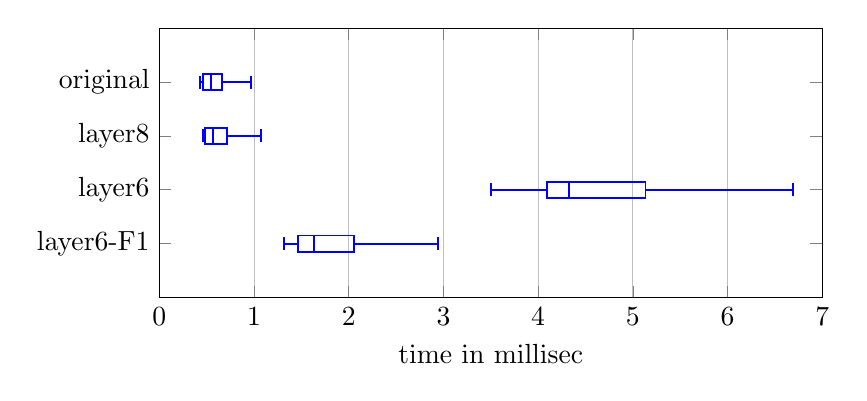
\begin{tikzpicture}
  \begin{axis} [
        %title={Time Comparison (n=4779 files)},
        height=5.0cm, width=10.0cm,
        xmajorgrids=true,
        xmin=0, xmax=7,
        ytick={1, 2, 3, 4},
        yticklabels={layer6-F1, layer6, layer8, original},
        legend style={at={(0.5,-0.2)}, anchor=north, legend columns=-1},
        ymin=0,ymax=5,
        xlabel= {time in millisec},
        /pgfplots/boxplot/box extend=0.3
    ]
    \addplot+ [ % original
    color=blue,
    line width=0.7pt,
    boxplot prepared={
      median=0.5409755,
      upper quartile=0.6654755,
      lower quartile=0.4631035,
      upper whisker=0.9667040,
      lower whisker=0.4266190,
      draw position=4,
    },
    ] coordinates {};
    \addplot+ [ % layer8
    color=blue,
    line width=0.7pt,
    boxplot prepared={
      median=0.5651665,
      upper quartile=0.7184590,
      lower quartile=0.4821770,
      upper whisker=1.0725120,
      lower whisker=0.4605160,
      draw position=3
    },
    ] coordinates {};
    \addplot+ [ % layer6
    color=blue,
    line width=0.7pt,
    boxplot prepared={
      median=4.3254265,
      upper quartile=5.1334505,
      lower quartile=4.09074675,
      upper whisker=6.6958220,
      lower whisker=3.5065080,
      draw position=2
    },
    ] coordinates {};
    \addplot+ [ % layer6-F1
    color=blue,
    line width=0.7pt,
    boxplot prepared={
      median=1.6361880,
      upper quartile=2.05605575,
      lower quartile=1.4636370,
      upper whisker=2.9433810,
      lower whisker=1.3118650,
      draw position=1
    },
    ] coordinates {};
  \end{axis}
\end{tikzpicture}
\end{document}
